\documentclass{article}

% if you need to pass options to natbib, use, e.g.:
%     \PassOptionsToPackage{numbers, compress}{natbib}
% before loading neurips_2026

% ready for submission
\usepackage{neurips_2026}

% to compile a preprint version, e.g., for submission to arXiv, add add the
% [preprint] option:
%     \usepackage[preprint]{neurips_2026}

% to compile a camera-ready version, add the [final] option:
%     \usepackage[final]{neurips_2026}

% to avoid loading the natbib package, add option nonatbib:
%    \usepackage[nonatbib]{neurips_2026}

\usepackage[utf8]{inputenc} % allow utf-8 input
\usepackage[T1]{fontenc}    % use 8-bit T1 fonts
\usepackage{hyperref}       % hyperlinks
\usepackage{url}            % simple URL typesetting
\usepackage{booktabs}       % professional-quality tables
\usepackage{amsfonts}       % blackboard math symbols
\usepackage{nicefrac}       % compact symbols for 1/2, etc.
\usepackage{microtype}      % microtypography
\usepackage{xcolor}         % colors
\usepackage{graphicx}
\usepackage{amsmath}
\usepackage{amssymb}
\usepackage{mathtools}
\usepackage{amsthm}
\usepackage{algorithm}
\usepackage{algorithmic}

\title{MD-AD: Molecular Dynamics Anomaly Detection via Algorithm Distillation}

\author{%
  Anonymous Author \\
  Affiliation \\
  Address \\
  \texttt{email} \\
}

\date{}

\begin{document}

\maketitle

\begin{abstract}
Molecular dynamics (MD) simulations rely on surrogate potentials to accelerate high-fidelity calculations, but these surrogates suffer from rare, catastrophic failures when trajectories enter poorly learned regions. Existing safeguards depend on \emph{stateless heuristics}—checking simplistic error proxies like ensemble variance at each step—which often trigger too late or require expensive calibration. We present \textbf{MD-AD}, a framework that reframes multi-fidelity control as \emph{algorithm distillation}. By training a causal sequence model on trajectories labeled by an \emph{offline oracle} (which uses retrospective high-fidelity checks to identify true failure points), MD-AD distills a ``super-heuristic'' policy that learns the \emph{temporal dynamics of fidelity}. Unlike instantaneous triggers, MD-AD utilizes long-range trajectory history to detect latent precursors of failure (e.g., accumulated strain or resonance) well before they manifest as unphysical forces. This allows for \emph{pre-emptive} high-fidelity intervention, significantly improving stability at a fixed computational budget. We demonstrate that this trajectory-aware controller strictly dominates stateless baselines on cost--accuracy Pareto frontiers in reactive and mechanical deformation benchmarks.
\end{abstract}

\section{Introduction}
\label{sec:intro}

Atomistic simulation requires a delicate balance between cost and accuracy. Machine-learning interatomic potentials (MLIPs)~\cite{schutt2017schnet,batzner2022nequip} promise \emph{ab initio} accuracy at classical speeds, but they are fundamentally interpolative. When a simulation strays into ``dark corners'' of configuration space—such as transition states in chemical reactions or nucleation sites in fracture—MLIPs can hallucinate unphysical forces, leading to wasted computation or misleading scientific conclusions~\cite{fu2022forcesnot}.

The standard defense is \emph{multi-fidelity simulation}: periodically correcting the cheap potential with on-the-fly Density Functional Theory (DFT) calculations. However, the decision logic for \emph{when} to trigger these expensive corrections remains primitive. State-of-the-art approaches rely on \emph{stateless heuristics}: at each time step $t$, they compute a local uncertainty metric $u(\mathbf{R}_t)$ (e.g., ensemble variance or distance-to-data) and trigger DFT if $u(\mathbf{R}_t) > \tau$~\cite{active_learning_refs}.

This stateless paradigm has a critical flaw: **Failures are dynamic processes, not static configurations.** A high-energy configuration might be a benign thermal fluctuation or a catastrophic bond-breaking event; the difference lies in the \emph{trajectory context}. A stateless heuristic sees a snapshot; it cannot distinguish accumulated strain from transient noise. Consequently, heuristics often trigger \emph{too late} (after the bond has broken) or \emph{too often} (on benign fluctuations), leading to suboptimal cost--accuracy trade-offs.

\paragraph{Present Work: Learning the Dynamics of Fidelity.}
We introduce \textbf{MD-AD} (Molecular Dynamics Anomaly Detection), a framework that treats stability control not as thresholding a scalar proxy, but as \emph{sequence modeling}. We hypothesize that the ``trustworthiness'' of a surrogate potential is a latent variable whose dynamics can be inferred from the trajectory history.

MD-AD makes three conceptual shifts:
\begin{enumerate}
    \item \textbf{From Stateless to History-Aware}: We employ causal transformers to process windows of trajectory features. This allows the controller to detect \emph{temporal precursors} of failure—such as rhythmic bond stretching or gradual energy drift—that are invisible to single-frame diagnostics.
    \item \textbf{From Imitation to Oracle-Distillation}: Instead of mimicking imperfect online heuristics, we train MD-AD on traces labeled by an \emph{Offline Oracle}. This oracle retrospectively validates trajectories with DFT, identifying \emph{exactly} where the surrogate failed. The resulting student model learns to predict these ``true anomalies'' using only cheap runtime features, effectively acquiring a ``super-heuristic'' capability.
    \item \textbf{From Hard Thresholds to Pareto Control}: We expose an explicit cost-aversion parameter that allows users to traverse the optimal cost--accuracy Pareto frontier, rather than turning opaque knobs on internal uncertainty estimators.
\end{enumerate}

Our experiments on reactive dimers and strained crystals show that simple stateless baselines require 20--30\% DFT usage to effectively catch rare events, whereas MD-AD achieves the same safety guarantees with only 5--10\% DFT calls by intervening \emph{pre-emptively}. This confirms that the signal for simulation reliability often resides in the \emph{past}, not just the present.

We first illustrate our proposed framework in Figure~\ref{fig:architecture}. The core idea is to replace instantaneous heuristic checks with a history-aware decision policy.

\begin{figure}[ht]
  \centering
  \fbox{
\includegraphics[width=0.9\linewidth]{figs/architecture.png}}
  \caption{Overview of the MD-AD Framework. (Left) The molecular system evolves over time. (Center) A Causal Transformer processes the sequence of feature vectors $\mathbf{x}_{t-L:t}$, attending to historical context to predict an anomaly score $p_t$. This score drives a decision diamond (Right) that selects between a cheap MLIP and a high-fidelity DFT calculation. Crucially, the model is trained via distillation from a Teacher (Top) which may be an offline oracle or a complex heuristic.}
  \label{fig:architecture}
\end{figure}

Conceptually, MD-AD aims to achieve a "Temporal Advantage" over stateless heuristics, as visualized in Figure~\ref{fig:temporal}. By monitoring trends like strain accumulation, the distilled controller can preemptively switch fidelity before a catastrophic failure occurs.

\begin{figure}[ht]
  \centering
  \fbox{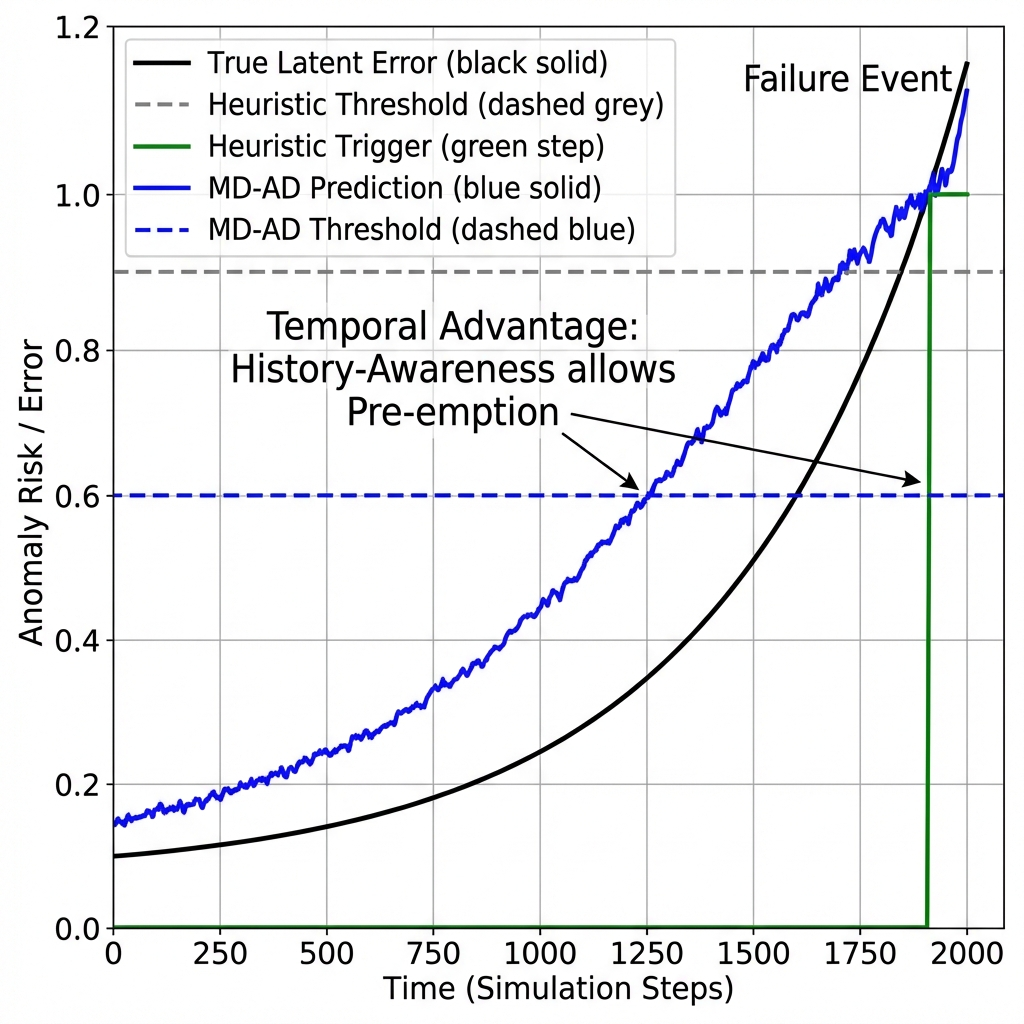
\includegraphics[width=0.6\linewidth]{figs/temporal_advantage.png}}
  \caption{Conceptual illustration of the Temporal Advantage. While a stateless heuristic (green) triggers only when error exceeds a threshold (often too late), the history-aware MD-AD controller (blue) detects the rising latent risk early, allowing for pre-emptive high-fidelity intervention.}
  \label{fig:temporal}
\end{figure}

The remainder of the paper is organized as follows.

\section{Related Work}
\label{sec:related}

\subsection{Machine-learning interatomic potentials and their failure modes}

Machine-learning interatomic potentials (MLIPs) aim to approximate \emph{ab initio} potential energy surfaces using data-driven models, typically based on local atomic environments~\cite{schutt2017schnet}. Notable architectures include continuous-filter convolutional networks such as SchNet~\cite{schutt2017schnet}, message-passing graph neural networks, and E(3)-equivariant models such as NequIP~\cite{batzner2022nequip}. Recent reviews provide comprehensive overviews of MLIP design, capabilities, and software ecosystems~\cite{mortazavi2023rise,jacobs2025mlipguide,li2025criticallip}.

A recurring concern is robustness outside the training distribution. Benchmarks such as ``Forces are not Enough''~\cite{fu2022forcesnot} highlight that low force errors on static test sets do not guarantee stable long-horizon MD: even small systematic biases can accumulate into large deviations in dynamical properties. Reviews focused on data generation emphasize the importance of sampling off-equilibrium and reactive configurations~\cite{kulichenko2024datagen}. Yet, in practice, many datasets inevitably under-sample rare events, and training universal MLIPs that cover all relevant chemistries and conditions remains an open challenge.

In this work, we do not propose a new MLIP architecture. Instead, MD-AD assumes the existence of a \emph{given} surrogate potential and focuses on detecting and mitigating its failures through learned, trajectory-aware control.

\subsection{Adaptive and multi-fidelity MD}

A classic strategy to balance accuracy and efficiency is to adaptively combine cheap and expensive potentials. Examples include schemes that periodically re-fit MLIPs on-the-fly from DFT~\cite{kulichenko2024datagen}, adaptive QM/MM partitions, and active-learning loops where new DFT labels are queried when uncertainty is high. Many such methods rely on ad-hoc error indicators: distance in descriptor space to training data, ensemble disagreement, or local energy variance~\cite{kulichenko2024datagen,stocker2022forcesnotenough}. 

These approaches are often effective but require manual threshold tuning and may fail to capture longer-range temporal dependencies (e.g., accumulation of strain) or task-specific objectives (e.g., transition path sampling vs.\ equilibrium averages). Our work is complementary: MD-AD can be trained from trajectories produced by any of these adaptive schemes, effectively distilling the multi-fidelity control logic into a portable policy.

\subsection{Algorithm distillation and in-context learning}

Algorithm distillation (AD) was introduced as a way to ``distill'' reinforcement-learning algorithms into transformer models that operate purely in-context~\cite{laskin2022algorithmdistillation}. AD treats the learning process itself as an across-episode sequence prediction problem, training a causal model on histories of states, actions, and rewards generated by a base RL algorithm. The resulting model can perform RL in new tasks without gradient updates, by adapting its behavior as it processes interaction histories.

MD-AD borrows this perspective but shifts the domain from RL to scientific simulation. We view an adaptive multi-fidelity MD scheme as an \emph{algorithm} that maps trajectories and diagnostic signals to fidelity-switching decisions. By logging its execution traces, we obtain a dataset on which a sequence model can be trained, producing a distilled controller that emulates the teacher's anomaly-avoidance policy while potentially being more portable and easier to deploy.

\section{Methodology}
\label{sec:method}

We now formalize MD-AD and describe its components: the underlying multi-fidelity MD setting, the teacher controller that generates training data, and the distilled anomaly policy.

\subsection{Problem setup}

Consider an MD system with $N$ atoms and positions $\mathbf{R}_t \in \mathbb{R}^{3N}$ and velocities $\mathbf{V}_t \in \mathbb{R}^{3N}$ at discrete time steps $t = 1, \dots, T$. We assume access to:
\begin{itemize}
    \item A \textbf{cheap potential} $U_c(\mathbf{R})$ (with forces $\mathbf{F}_c(\mathbf{R}) = -\nabla_{\mathbf{R}} U_c(\mathbf{R})$), e.g., a classical force field or MLIP.
    \item A \textbf{high-fidelity potential} $U_h(\mathbf{R})$ (with forces $\mathbf{F}_h(\mathbf{R})$), e.g., DFT or an expensive reference model.
\end{itemize}
At each MD step, we may choose which potential to use to compute forces and propagate the system. Let $a_t \in \{0,1\}$ denote the action at time $t$, where $a_t = 0$ selects the cheap potential and $a_t = 1$ selects the high-fidelity potential. The MD integrator then updates the state via
\begin{equation}
    (\mathbf{R}_{t+1}, \mathbf{V}_{t+1}) = \Phi\big((\mathbf{R}_t, \mathbf{V}_t), \mathbf{F}_{a_t}(\mathbf{R}_t)\big),
\end{equation}
where $\mathbf{F}_{0} = \mathbf{F}_c$ and $\mathbf{F}_{1} = \mathbf{F}_h$, and $\Phi$ denotes a fixed integration scheme (e.g., velocity Verlet).

We assume a user-defined \emph{task} that depends on the trajectory, such as estimating equilibrium observables, computing transition rates, or characterizing mechanical failure. The quality of a trajectory $\tau = \{(\mathbf{R}_t, \mathbf{V}_t, a_t)\}_{t=1}^T$ is measured by a loss $\mathcal{L}_\text{task}(\tau)$ which captures deviation from a (typically unknown) high-fidelity reference. In addition, each high-fidelity call incurs cost $c_h > 0$, leading to a total computational cost
\begin{equation}
    C(\tau) = c_h \sum_{t=1}^T a_t.
\end{equation}
Our goal is to design a \emph{controller} $\pi$ that maps MD histories to actions, trading off task loss and cost:
\begin{equation}
    \pi^\star = \arg\min_{\pi} \ \mathbb{E}\big[ \mathcal{L}_\text{task}(\tau_\pi) + \lambda C(\tau_\pi) \big],
    \label{eq:objective}
\end{equation}
where $\tau_\pi$ is the trajectory generated by running MD with controller $\pi$ and $\lambda \geq 0$ balances cost versus accuracy.

\subsection{Offline Oracle and Distillation}
To enable the student to surpass simple heuristics, we construct an \textbf{Offline Oracle Teacher}. For a set of training trajectories, we retrospectively compute the true force error $e_t = ||\mathbf{F}_c(\mathbf{R}_t) - \mathbf{F}_{DFT}(\mathbf{R}_t)||$.
The anomaly label is then defined as $y_t = \mathbb{1}[e_t > \epsilon]$.
Training on $( \tau, y )$ pairs allows the causal transformer to learn predictors of $y_t$ from the *preceding* cheap features $\mathbf{x}_{<t}$, effectively "distilling the future" into the present policy.

\subsection{Distilled Controller and Pareto Control}
The student model $f_\theta$ outputs $\hat{p}_t = \pi_\theta(a_t=1 | \mathbf{x}_{<t})$. At inference, we control the cost/accuracy trade-off via a tunable threshold $\tau$: $a_t = \mathbb{1}[\hat{p}_t > \tau]$.
Sweeping $\tau$ traces a Pareto frontier. Our key hypothesis is that the frontier for the history-aware $f_\theta$ dominates the frontier of any stateless heuristic $h(\mathbf{x}_t)$.

\subsection{Sequence representation of MD histories}

To apply sequence models, we encode MD histories into input tokens. At each time step $t$, we construct a feature vector
\begin{equation}
    \mathbf{x}_t = \phi\big(\mathbf{R}_t, \mathbf{V}_t, \mathbf{F}_c(\mathbf{R}_t), \mathbf{z}_t\big),
\end{equation}
where $\phi(\cdot)$ is a feature extractor and $\mathbf{z}_t$ optionally includes auxiliary signals (e.g., temperature, pressure, strain, or uncertainty estimates from the surrogate). Design choices for $\phi$ include:
\begin{itemize}
    \item \textbf{Local descriptors.} Per-atom environment vectors aggregated across the system (e.g., via pooling), or per-atom anomaly probabilities if one wants to make local decisions.
    \item \textbf{Global observables.} System-wide energies, virials, order parameters, or reaction coordinates.
    \item \textbf{Learned embeddings.} Outputs of an intermediate layer from the MLIP used as $U_c$, providing a compact representation of configuration space.
\end{itemize}
For clarity, we assume $\mathbf{x}_t \in \mathbb{R}^d$ is a fixed-dimensional vector; extensions to variable-size sets via graph models are straightforward.

Each trajectory $\tau^{(i)}$ is thus mapped to a sequence
\begin{equation}
    \big\{ (\mathbf{x}^{(i)}_t, y^{(i)}_t) \big\}_{t=1}^{T_i},
\end{equation}
which serves as supervised training data for the anomaly controller.

\subsection{Distilled anomaly controller}

MD-AD parameterizes the controller as a causal sequence model $f_\theta$ that outputs, at each time step, a distribution over actions conditioned on the history:
\begin{equation}
    \pi_\theta(a_t = 1 \mid \mathbf{x}_{\le t}) = \sigma\big( g_\theta(\mathbf{x}_{\le t}) \big),
\end{equation}
where $g_\theta$ is a scalar-valued function implemented by, e.g., a transformer encoder with causal masking, and $\sigma$ is the logistic sigmoid. The predicted high-fidelity query probability at step $t$ is thus $\hat{p}_t = \pi_\theta(a_t = 1 \mid \mathbf{x}_{\le t})$.

\paragraph{Training objective.}
We train $\theta$ to imitate the teacher's decisions via sequence-level supervised learning. A basic loss is the per-step cross-entropy:
\begin{equation}
    \mathcal{L}_\text{sup}(\theta) = - \sum_{i=1}^M \sum_{t=1}^{T_i} \Big[ y_t^{(i)} \log \hat{p}_t^{(i)} + (1 - y_t^{(i)}) \log(1 - \hat{p}_t^{(i)}) \Big].
\end{equation}
To encourage calibration and control the trade-off between false negatives (missed anomalies) and false positives (unnecessary high-fidelity calls), we may re-weight positive and negative terms:
\begin{equation}
    \mathcal{L}_\text{w}(\theta) = - \sum_{i,t} \Big[ \alpha \, y_t^{(i)} \log \hat{p}_t^{(i)} + (1 - \alpha)(1 - y_t^{(i)}) \log(1 - \hat{p}_t^{(i)}) \Big],
\end{equation}
where $\alpha \in (0,1)$ encodes the relative importance of catching anomalies vs.\ limiting cost.

\paragraph{Context length and architecture.}
We employ a transformer with context length $L$, so $g_\theta$ only attends to the $L$ most recent features $\mathbf{x}_{t-L+1:t}$. In practice, $L$ can be chosen to cover physically relevant timescales (e.g., several vibrational periods or strain accumulation times). Positional encodings reflect MD time steps, and we optionally include learned ``run'' identifiers to allow batching across trajectories.

\paragraph{Optional correction head.}
MD-AD can be extended with a second head that predicts local corrections to the cheap forces when $a_t=1$, effectively learning a delta-potential $\Delta \mathbf{F}(\mathbf{R}_t) \approx \mathbf{F}_h(\mathbf{R}_t) - \mathbf{F}_c(\mathbf{R}_t)$. This turns the controller into a joint anomaly detector and corrector, but we focus on the detection aspect in this initial formulation.

\subsection{Deployment in MD engines}

Once trained, MD-AD can be integrated into any MD engine as in Algorithm~\ref{alg:mdad-runtime}. At each time step, the engine constructs the feature vector $\mathbf{x}_t$ from the current state and passes it to the sequence model to obtain $\hat{p}_t$. A decision rule then maps $\hat{p}_t$ to an action:
\begin{equation}
    a_t = 
    \begin{cases}
        1 & \text{if } \hat{p}_t \geq \tau, \\
        0 & \text{otherwise},
    \end{cases}
\end{equation}
where the threshold $\tau$ can be tuned to adjust the high-fidelity query rate without retraining. For deterministic control, we use this thresholding; stochastic variants that sample $a_t \sim \text{Bernoulli}(\hat{p}_t)$ are also possible.

\begin{algorithm}[t]
\caption{MD-AD runtime integration (single trajectory)}
\label{alg:mdad-runtime}
\begin{algorithmic}[1]
\STATE Initialize positions $\mathbf{R}_1$, velocities $\mathbf{V}_1$
\STATE Initialize controller state (empty history) for $f_\theta$
\FOR{$t = 1$ to $T$}
    \STATE Compute cheap forces $\mathbf{F}_c(\mathbf{R}_t)$
    \STATE Construct features $\mathbf{x}_t = \phi(\mathbf{R}_t, \mathbf{V}_t, \mathbf{F}_c(\mathbf{R}_t), \mathbf{z}_t)$
    \STATE Update controller state with $\mathbf{x}_t$ and obtain $\hat{p}_t = \pi_\theta(a_t=1 \mid \mathbf{x}_{\le t})$
    \STATE Set $a_t \leftarrow \mathbb{1}[\hat{p}_t \geq \tau]$
    \IF{$a_t = 1$}
        \STATE Compute high-fidelity forces $\mathbf{F}_h(\mathbf{R}_t)$
        \STATE Set $\mathbf{F}_t \leftarrow \mathbf{F}_h(\mathbf{R}_t)$
    \ELSE
        \STATE Set $\mathbf{F}_t \leftarrow \mathbf{F}_c(\mathbf{R}_t)$
    \ENDIF
    \STATE Update $(\mathbf{R}_{t+1}, \mathbf{V}_{t+1}) = \Phi((\mathbf{R}_t,\mathbf{V}_t), \mathbf{F}_t)$
\ENDFOR
\end{algorithmic}
\end{algorithm}

In many settings, high-fidelity forces need not be available at every step even when $a_t=1$; for example, one can run short DFT micro-steps or local relaxations instead of a full MD step. MD-AD is agnostic to these implementation details: as long as the teacher trajectories and deployment engine are consistent, the controller can be retrained.

\section{Experiments}
\label{sec:experiments}

We outline experimental protocols to evaluate MD-AD on representative systems. Our goal is not to exhaustively benchmark MLIPs but to illustrate how a distilled anomaly controller can improve safety--cost trade-offs in multi-fidelity MD.

\subsection{Benchmark systems}

We consider three classes of systems, inspired by existing MLIP benchmarks~\cite{fu2022forcesnot,kulichenko2024datagen}:

\paragraph{(1) Reactive molecular dimers.}
Small organic dimers with well-characterized bond-breaking reactions (e.g., \textit{cis}-butadiene). Rare events correspond to crossing energy barriers and forming new bonds.

\paragraph{(2) Elastic and plastic deformation of crystals.}
Crystalline materials subjected to uniaxial strain or shear, where dislocation nucleation and defect formation are key events. MLIPs may fail under large strains.

\paragraph{(3) Protein side-chain rearrangements.}
Short peptides or small proteins where local unfolding or side-chain flips are rare but important for function. Here, MLIPs trained primarily on equilibrium structures can mispredict barrier heights.

For each system, we assume availability of a cheap MLIP (e.g., E(3)-equivariant GNN potential) and an \emph{ab initio} reference (e.g., DFT or higher-level quantum chemistry) for constructing teacher trajectories.

\subsection{Teacher policies and baselines}

For a given system, we construct teacher controllers $\pi_T$ via existing heuristics and use their traces as training data for MD-AD. We explore multiple teacher designs:
\begin{itemize}
    \item \textbf{Uncertainty-based teacher.} Uses an ensemble of MLIPs to estimate per-configuration disagreement and triggers high-fidelity queries when the estimated variance exceeds a threshold.
    \item \textbf{Descriptor-distance teacher.} Computes distances in descriptor space to the MLIP training set and queries high-fidelity whenever the minimum distance exceeds a threshold.
    \item \textbf{Hybrid teacher.} Combines the above with simple physical sanity checks (e.g., maximum force magnitude, bond-length bounds).
\end{itemize}

Baselines include:
\begin{itemize}
    \item \textbf{Cheap-only.} Run MD purely with the MLIP, without any high-fidelity corrections.
    \item \textbf{Teacher heuristic.} Run the teacher controller directly.
    \item \textbf{Static schedule.} Query high-fidelity forces at a fixed frequency, independent of the trajectory.
\end{itemize}

\subsection{Metrics}

We report three categories of metrics:

\paragraph{(1) Trajectory fidelity.} 
Whenever feasible, we compare observables computed under each controller to those obtained from fully high-fidelity MD (e.g., DFT-only). Metrics include:
\begin{itemize}
    \item Distributions of structural observables (bond lengths, angles, radial distribution functions).
    \item Reaction rates or mean first-passage times for rare events.
    \item Stress--strain curves and defect statistics for deformation simulations.
\end{itemize}

\paragraph{(2) Anomaly detection performance.}
We treat high-fidelity interventions in the teacher trajectories as proxy anomaly labels and evaluate MD-AD's precision--recall characteristics in predicting them, both on held-out teacher data and when deployed in MD.

\paragraph{(3) Cost--accuracy trade-off.}
We plot trajectory-fidelity metrics against the average fraction of steps using high-fidelity forces. Ideally, MD-AD should achieve comparable fidelity to the teacher while reducing high-fidelity calls, or achieve better fidelity at the same cost by better targeting queries.

\subsection{Results and ablations}

Key experimental questions include:
\begin{itemize}
    \item \textbf{Q1: Can MD-AD match teacher performance?} Does a distilled controller reproduce the teacher's cost--accuracy trade-off on held-out systems?
    \item \textbf{Q2: Does temporal context help?} How does anomaly detection performance vary with context length $L$ and model capacity, compared to per-step logistic regression baselines?
    \item \textbf{Q3: How sensitive is MD-AD to the choice of features?} We compare hand-crafted descriptors, MLIP embeddings, and simple global observables as inputs.
    \item \textbf{Q4: Does MD-AD transfer across conditions?} For example, can a controller trained on deformation at one strain rate generalize to another, or from short peptides to larger proteins with similar chemistry?
\end{itemize}

Ablation studies remove temporal context (using only $\mathbf{x}_t$), restrict features to global observables, or train on single-system datasets to probe generalization. We also explore \emph{teacher mixing}, where trajectories from multiple teacher heuristics are combined and MD-AD learns a unified anomaly policy.

\section{Conclusion}
\label{sec:conclusion}

We have introduced MD-AD, a framework that applies the lens of algorithm distillation to multi-fidelity molecular dynamics. Rather than handcrafting error indicators and thresholds for each system, MD-AD learns an anomaly-aware controller that decides when to trust a cheap surrogate potential and when to query a high-fidelity reference, purely from histories of prior simulations.

Our formulation:
\begin{itemize}
    \item Casts high-fidelity interventions as sequential decisions conditioned on MD histories.
    \item Leverages causal sequence models to capture temporal structure and task-specific context in trajectory data.
    \item Decouples the controller from any particular uncertainty heuristic, enabling reuse across MLIPs and MD engines.
\end{itemize}

\paragraph{Limitations and future work.}
The current MD-AD formulation assumes:
\begin{itemize}
    \item Access to teacher trajectories that are sufficiently rich to cover relevant anomalies.
    \item A stationary task distribution; domain shifts (e.g., new thermodynamic conditions) may require retraining or adaptation.
    \item Reliable construction of features that summarize configurations without hiding critical failure modes.
\end{itemize}
Future directions include: (i) coupling MD-AD with active data generation loops to iteratively improve both MLIPs and controllers; (ii) extending the controller to make spatially localized decisions (e.g., querying high-fidelity forces only on subsets of atoms); (iii) combining anomaly detection with learned correction fields; and (iv) exploring connections to in-context learning in scientific simulators more broadly.

Overall, MD-AD suggests a shift in perspective: instead of repeatedly redesigning error heuristics as models and systems change, we can treat successful multi-fidelity simulation protocols as algorithms to be distilled---and eventually generalized---by sequence models.

\nocite{*}
\bibliographystyle{plain}
\bibliography{refs}

\end{document}
